\subsection{Sistem Kontrol Adaptif dengan Model Prediktif berbasis \textit{Time Series}}

Seperti yang sudah dijelaskan pada bagian rancangan solusi (\ref{sec:rancangan-solusi}), sistem kontrol adaptif akan diimplementasikan dengan beberapa komponen penyusun, diantaranya adalah sebagai berikut.

\subsubsection{Komponen \textit{Metrics Fetcher}}
\textbf{\textit{Metrics Fetcher}} merupakan komponen yang berbeda dibanding komponen lainnya, karena komponen ini berjalan pada \textit{script} serta proses yang berbeda. Seperti yang sudah dijelaskan sebelumnya, komponen ini akan menembak permintaan HTTP pada \href{https://www.elastic.co/guide/en/elasticsearch/reference/current/cluster-nodes-stats.html}{\textit{Node Stats API}} yang telah disediakan \textit{Elastic Search} lalu melakukan transformasi bentuk data menjadi bentuk yang lebih sederhana dan sesuai kebutuhan. Komponen ini akan berjalan pada \textit{script} yang berbeda dikarenakan bahasa Python memiliki kekurangan dalam penanganan \textit{multithreading}. Komponen ini akan mengirimkan data yang sudah diolah ke komponen \textbf{\textit{Predictor}} melalui \textit{stream file}. Pendekatan ini dipilih karena sederhana dan mudah diimplementasikan. Khusus komponen ini, struktur kodenya tidak memakai sistem kelas dan hanya terdapat sebuah fungsi dan beberapa baris perintah untuk melakukan pemanggilan API, transformasi data dan pengiriman data ke \textit{stream file}.

\subsubsection{Komponen \textit{Predictor}}
Komponen \textbf{\textit{Predictor}} terdiri dari 3 buah kelas, yaitu sebagai berikut.
\begin{enumerate}
    \item \textbf{\textit{Predict Component}}
    
    Kelas ini berfungsi untuk menyimpan sebuah model ARIMA untuk sebuah variabel. Kelas ini memanfaatkan kakas pandas, statsmodels dan pmdarima untuk melakukan tanggung jawabnya.

    \item \textbf{\textit{Predict Component Factory}}
    
    Kelas ini berfungsi untuk membuat objek \textbf{\textit{Predict Component}} sebanyak variabel yang ada. 

    \item \textbf{\textit{Predict Component Storage}}
    
    Kelas ini berfungsi sebagai aggregator objek \textbf{\textit{Predict Component}} yang telah dibuat oleh \textbf{\textit{Predict Component Factory}}. Kelas ini juga berfungsi untuk meneruskan sebuah aksi kepada semua objek \textbf{\textit{Predict Component}} yang ada. Contohnya, dengan memanggil \textit{forecast} atau \textit{update data}, maka operasi akan diteruskan ke semua objek \textbf{\textit{Predict Component}}.

\end{enumerate}

\begin{figure}[h]
    \centering
    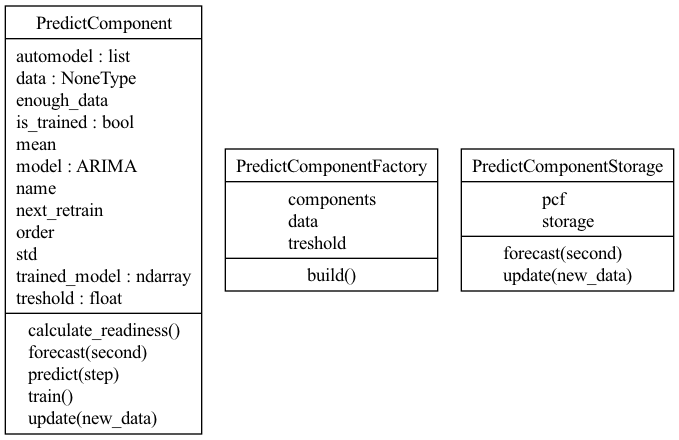
\includegraphics[width=0.8\textwidth]{chapter-4/predictor.png}
    \caption{Spesifikasi Kelas Penyusun Komponen \textit{Predictor}}
    \label{fig:predictor-spek}
\end{figure}

Secara umum, spesifikasi kelas bisa dilihat pada gambar \ref{fig:predictor-spek}. Kelas \textbf{\textit{Predict Component Storage}} akan membutuhkan \textbf{\textit{Predict Component Factory}} untuk membangun semua \textbf{\textit{Predict Component}} untuk setiap variabel yang ada. Setelah itu, terdapat operasi seperti meneruskan penambahan data serta meminta data prediksi ke setiap \textbf{\textit{Predict Component}}. Kelas ini akan digunakan oleh komponen \textbf{\textit{Adaptive Control}} untuk lebih lanjutnya.

\subsubsection{Komponen \textit{Rule Manager}}
Komponen \textbf{\textit{Rule Manager}} berfungsi untuk melakukan parsing terhadap file \textit{rule} yang telah diisi oleh pengguna serta menjadi aggregator untuk melakukan pengecekan \textit{rule} yang berlangsung serta memberi informasi data prediksi kapan saja yang dibutuhkan untuk melakukan pengecekan. Parsing komponen ini menggunakan format csv dan kondisi diekspresikan dengan sintaks python. Komponen ini akan menghasilkan sebuah objek \textbf{\textit{Rule}} yang akan digunakan oleh komponen \textbf{\textit{Adaptive Control}}. Agar terbayang, contoh dari \textit{file rule} dapat dilihat pada lampiran XXX. Spesifikasi dari kedua kelas tersebut dapat dilihat pada gambar \ref{fig:rule-spek}.

% TODO CONTOH RULE, masukin ke lampiran, trus tag kesini.

Sebuah \textit{rule} memiliki fungsi sebagai berikut.
\begin{enumerate}
    \item Memiliki sebuah kondisi yang akan dievaluasi dengan data prediksi pada waktu prediksi yang diinginkan. Contoh: kondisi \textit{throughput} untuk operasi X untuk 1 menit kedepan dan 5 menit kedepan lebih dari 1s, maka tingkatkan prosesor sebanyak 500m.
    \item Memiliki jumlah serta target kategori untuk diubah, dalam kasus ini pilihannya memori atau prosesor.
    \item Satuan untuk perubahan memori adalah dalam \textit{Mebibyte} atau MiB. Sedangkan untuk prosesor dalam satuan mili atau m.
    \item Sebuah \textit{rule} memiliki periode pengecekan sehingga tidak akan dicek secara terus menerus yang menyebabkan perubahan alokasi sumber daya terlalu cepat. Periode pengecekan dibuat dalam satuan sekon.
\end{enumerate}

\begin{figure}[h]
    \centering
    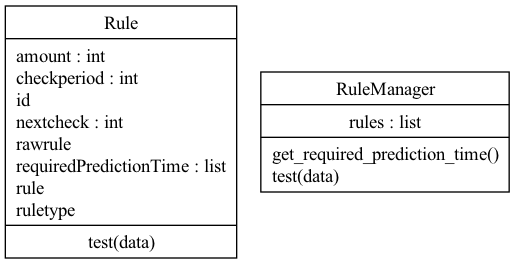
\includegraphics[width=0.8\textwidth]{chapter-4/rule.png}
    \caption{Spesifikasi Kelas Penyusun Komponen \textit{Rule Manager}}
    \label{fig:rule-spek}
\end{figure}

\subsubsection{Komponen \textit{Resource Controller}}

Komponen ini terdiri dari sebuah kelas. Seperti namanya, kelas ini berfungsi untuk menggunakan \textit{Kubernetes Client API} untuk mengubah alokasi sumber daya. Kelas ini diimplementasikan dengan sistem antrian, sehingga jika sejumlah rule aktif secara bersamaan, maka akan dijalankan secara berurutan. Terdapat sebuah fungsi \textit{tick} yang akan berfungsi untuk mengeksekusi antrian. Spesifikasi kelas ini dapat dilihat pada gambar \ref{fig:rc-spek}.

\begin{figure}[h]
    \centering
    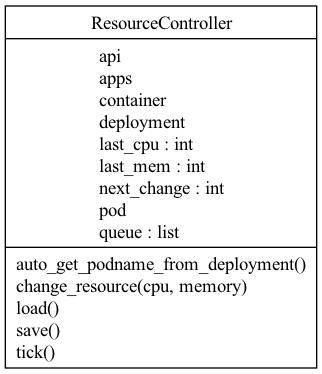
\includegraphics[width=0.8\textwidth]{chapter-4/rc.png}
    \caption{Spesifikasi Kelas Penyusun Komponen \textit{Resource Controller}}
    \label{fig:rc-spek}
\end{figure}

\subsubsection{Komponen \textit{Adaptive Control}}

\textbf{\textit{Adaptive Control}} mengkolaborasikan \textbf{\textit{Rule Manager}}, \textbf{\textit{Resource Controller}}, \textbf{\textit{Predict Component Factory}} dan \textbf{\textit{Predict Component Storage}}. Komponen ini akan meminta list waktu prediksi yang diperlukan dari \textbf{\textit{Rule Manager}} untuk \textbf{\textit{Rule Manager}} sehingga \textbf{\textit{Predict Component Storage}} dapat menyediakan data prediksi. Setelah itu, semua \textbf{\textit{Rule}} yang memenuhi syarat akan langsung ditransformasikan dan dikirim ke komponen \textbf{\textit{Resource Controller}}. Selain itu, komponen ini juga bertanggung jawab meneruskan data ke \textbf{\textit{Predict Component Storage}} untuk melakukan penambahan data. Spesifikasi kelas ini dapat dilihat pada gambar \ref{fig:ac-spek}.

\begin{figure}[h]
    \centering
    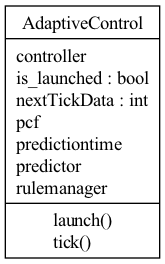
\includegraphics[width=0.8\textwidth]{chapter-4/ac.png}
    \caption{Spesifikasi Kelas Penyusun Komponen \textit{Adaptive Control}}
    \label{fig:ac-spek}
\end{figure}

\subsubsection{Lainnya: Konfigurasi dan Utilitas}

Seperti yang sudah dijelaskan sebelumnya, terdapat konfigurasi yang dapat mengatur sistem. Konfigurasi yang dapat diatur dapat dilihat pada gambar \ref{fig:config-spek}.

\begin{figure}[h]
    \centering
    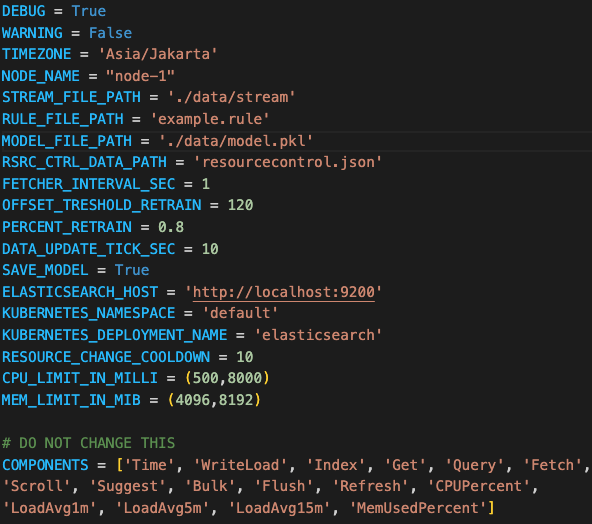
\includegraphics[width=0.8\textwidth]{chapter-4/config.png}
    \caption{Konfigurasi \textit{Adaptive Control}}
    \label{fig:config-spek}
\end{figure}

Setiap konfigurasi tersebut mengatur perilaku dari sistem. Untuk setiap konfigurasinya, berikut adalah penjelasannya.

\begin{enumerate}
    \item \textbf{\textit{Debug}} dan \textbf{\textit{Warning}}
    
    Kedua \textit{flag} ini adalah untuk mematikan dan menyalakan pesan \textit{debug} dan \textit{warning}. Jika \textit{debug} dimatikan, maka program tidak akan mengirimkan pesan apapun selama berjalan.

    \item \textbf{\textit{Timezone}}
    
    Untuk mengubah zona waktu yang digunakan oleh pandas. Karena data yang didapatkan dari \textit{Elastic Search} adalah berupa unix time sehingga akan dibaca \textit{default} menjadi UTC saat dikonversi. Flag ini berfungsi untuk mengubah zona waktu yang digunakan oleh pandas.

    \item \textbf{\textit{Node Name}}, \textbf{\textit{Namespace}} dan \textbf{\textit{Deployment Name}}
    
    \textbf{\textit{Node Name}} adalah nama \textit{node} yang telah dikonfigurasi pada \textit{elastic search}. Nama harus sesuai karena \textbf{\textit{Metrics Fetcher}} akan mencari data untuk node dengan nama tersebut. Sedangkan, \textbf{\textit{Namespace}} dan \textbf{\textit{Deployment Name}} berkaitan dengan \textit{namespace} dan \textit{deployment Elasticsearch} dengan Kubernetes.

    \item \textbf{\textit{Elasticsearch Host}}
    
    \textit{Flag} ini berisikan target \textit{host} dari \textit{Elasticsearch}. Bertindak sebagai \textit{Base URL} untuk mengakses API \textit{Elastic Search}.

    \item \textbf{\textit{CPU Limit}} dan \textbf{\textit{Memory Limit}}
    
    Kedua limit ini digunakan untuk \textbf{\textit{Resource Controller}} mengubah alokasi sumber daya. \textit{Flag} ini berisikan \textit{tuple} dengan dua buah angka yang berguna sebagai batas bawah dan batas atas dari sumber daya bersangkutan. Satuan yang digunakan untuk prosesor adalah mili (m) sedangkan untuk memori adalah \textit{mebibyte} (MiB). Kedua batas ini bersifat inklusif.

    \item \textbf{\textit{File Path}}
    
    Seperti namanya, konfigurasi yang berkaitan dengan \textit{file path} berfungsi untuk mengatur tata letak file yang akan dibuat/dibaca oleh sistem.

    \item \textbf{\textit{Fetcher Interval}}, \textbf{\textit{Resource Change Cooldown}} dan \textbf{\textit{Data Update Tick Second}}
    
    \textbf{\textit{Fetcher Interval}} adalah interval komponen \textbf{\textit{Metrics Fetcher}} melakukan penarikan data. Lalu, \textbf{\textit{Resource Change Cooldown}} adalah waktu yang diperlukan oleh \textbf{\textit{Resource Controller}} untuk menunggu sebelum melakukan perubahan sumber daya. Terakhir, \textbf{\textit{Data Update Tick Second}} adalah interval yang digunakan oleh \textbf{\textit{Adaptive Control}} untuk melakukan pembacaan data dari \textit{stream file}. \textbf{\textit{Data Update Tick Second}} harus lebih besar sama dengan \textbf{\textit{Fetcher Interval}} agar efisien. Satuan yang digunakan oleh ketiga \textit{flag} tersebut adalah detik.

    \item \textbf{\textit{Save Model}}
    
    \textit{Flag} ini berfungsi untuk mematikan penyimpanan model setiap kali model berubah. Jika \textit{flag} ini tidak dinyalakan, maka setiap kali sistem kontrol adaptif \textit{restart}, model prediksi akan diulang dari kosong.

    \item \textbf{\textit{Offset Treshold Retrain}} dan \textbf{\textit{Percent Retrain}}
    
    Dalam melakukan penambahan data, tidak setiap saat model akan di-\textit{retrain}. Saat tidak di-\textit{retrain}, model prediksi hanya melakukan update yang jauh lebih cepat namun tidak terlalu akurat. Terdapat sebuah angka yang akan menentukan kapan model harus di-\textit{retrain}. Hal ini diperlukan karena melakukan \textit{retrain} membutuhkan waktu yang lama terutama saat data sudah sangat besar. \textbf{\textit{Offset Treshold Retrain}} adalah angka yang menentukan kapan model harus di-\textit{retrain} berdasarkan jumlah data fixed. Sedangkan, \textbf{\textit{Percent Retrain}} adalah angka yang menentukan kapan model harus di-\textit{retrain} berdasarkan persentase jumlah data saat itu. Contohnya ketika saat ini data berukuran 100, dengan konfigurasi yang ada pada gambar \ref{fig:config-spek}, maka model akan di-\textit{retrain} ketika jumlah data sudah mencapai 200 atau 120+(80\% dari 100).
\end{enumerate}

Terdapat juga fungsi-fungsi utilitas yang akan membantu komponen-komponen yang telah dijelaskan sebelumnya, spesifikasi utilitas bisa dilihat pada gambar \ref{fig:util-spek}. Untuk setiap fungsinya, berikut adalah kegunaannya.

\begin{enumerate}
    \item \textbf{\textit{save model}}
    
    Fungsi ini akan menyimpan model yang telah dilatih ke dalam sebuah file. Digunakan kakas \textit{pickle} untuk melakukan hal ini.

    \item \textbf{\textit{load model}}
    
    Fungsi ini akan memuat model yang telah dilatih dari sebuah file. Digunakan kakas \textit{pickle} untuk melakukan hal ini.

    \item \textbf{\textit{timings}}
    
    Fungsi adalah abstraksi untuk menghitung waktu eksekusi. Digunakan fungsi sebagai \textit{return value} agar lebih rapih ketika diperlukan banyak penghitungan waktu eksekusi.

    \item \textbf{\textit{printd}}
    
    Fungsi ini hanyalah \textit{wrapper} dari fungsi \textit{print} pada Python untuk mengikuti aturan konfigurasi.

    \item \textbf{\textit{read from file}}
    
    Fungsi ini digunakan untuk membaca \textit{stream file}. Fungsi ini digunakan oleh komponen \textbf{\textit{Adaptive Control}} untuk membaca secara periodik, mentranformasikan dan mengirimkan data ke \textbf{\textit{Predict Component Storage}}.

    \item \textbf{\textit{to vector}}
    
    Fungsi ini adalah fungsi transformasi format JSON (\textit{Java Syntax Object Notation}) yang ditulis ke \textit{stream file} menjadi sebuah \textit{numpy array} yang akan digunakan untuk membuat \textit{pandas dataframe}.

    \item \textbf{\textit{create dataframe}}
    
    Seperti namanya, fungsi ini membuat dataframe dari data yang telah dibaca dari \textit{stream file} dan sudah ditransformasikan dengan fungsi \textbf{\textit{to vector}}.

    \item \textbf{\textit{extract number from string}}
    
    Fungsi ini memanfaatkan regex untuk mengambil angka dari sebuah string.
\end{enumerate}

\begin{figure}[h]
    \centering
    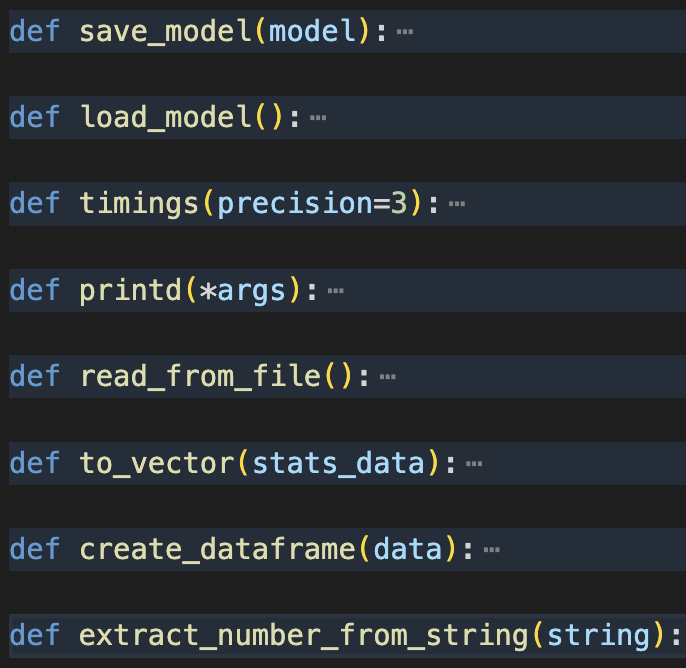
\includegraphics[width=0.8\textwidth]{chapter-4/utils.png}
    \caption{Spesifikasi Fungsi Utilitas Pendukung}
    \label{fig:util-spek}
\end{figure}

% TODO \subsubsection{Tampilan Implementasi}